\documentclass[12pt]{article}

\usepackage[utf8]{inputenc}
\usepackage[T1]{fontenc}
\usepackage{amsmath}
\usepackage{hyperref}
\usepackage{graphicx}

\graphicspath{{images/}}
\hypersetup{colorlinks=true, citecolor=blue}

\begin{document}

\title{Style Transfer in Text: Exploration and Evaluation}
\author{}
\date{}
\maketitle

\section{Idea}
The authors cite lack of parallel corpora and reliable evaluation metrics as the roadblocks for style transfer in natural language processing.

They aim to learn separate content representations and style representations, as is the case with pretty much any work dealing with style transfer in computer vision or natural language processing.

They measure 2 aspects of style transfer, namely transfer strength and content preservation.

\section{Method}
  \begin{itemize}
    \item The base method compared against is an autoencoder framework
    \item The authors employ 2 models:
    \begin{itemize}
      \item Multi-decoder seq2seq model \cite{sutskever2014sequence} that use the different decoders for different styles.
      \item Style-embeddings augmented decoder (single decoder) to generate outputs in different styles.
    \end{itemize}
    \item Adversarial objectives are applied to the content representation of both both. The objective is dissimilar to most adversarial objectives as it tries to maximize entropy of the predicted label from the content representation by minimizing $$-\sum_{i=1}^M\sum_{j=1}^N H(P(j|Encoder(x_i; \theta_e); \theta_c))$$ where $M$ is the size of the training data and $N$ is the number of distinct styles.
    \item Similar to the persona-based neural conversation model \cite{li2016persona}, a style embedding is learned for each different style. The conditional generation is done using recurrent neural networks with the inputs being the recurrent networks current state, and the style embedding to apply.
    \item The style embeddings matrix is not directly parameterized by the encoder, but the learning algorithm propagates changes based on how well it combines with the content representation to reconstruct the original text.
    \item The methods are evaluated in the following manner:
    \begin{itemize}
      \item Transfer strength is evaluated using a simple classifier
      \item Content preservation is evaluated by computing the cosine distance between the original and the generated text embeddings.
    \end{itemize}
  \end{itemize}

\section{Architecture}
  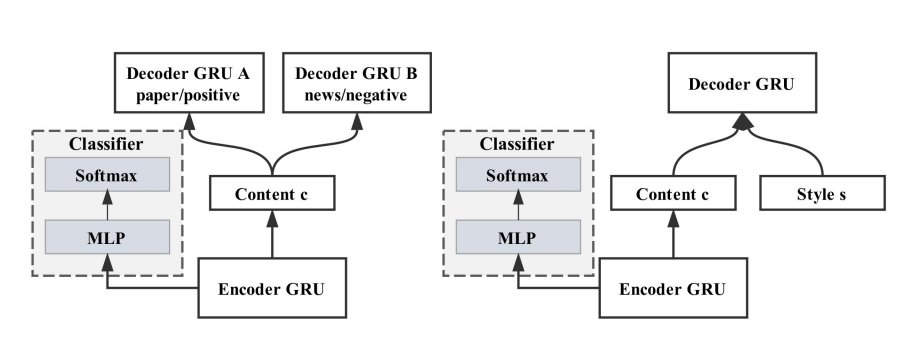
\includegraphics[width=\textwidth]{architecture}

\section{Observations}
  \begin{itemize}
    \item The authors don't explain:
    \begin{itemize}
      \item Why is a vanilla autoencoder the base model being compared with? It's objective does not optimize for transferring style.
      \item What ratings qualify as a positive/negative review?
      \item What kind of decoder strategy was used while predicting sequences? i.e. Greedy-search, Beam-search
      \item Which dictionary was used to filter sentimentally polar words for the evaluation.
    \end{itemize}
    \item The results indicate the the models proposed by the author in general perform better than the auto-encoder for the purposes of transfer strength.
    \item Although most of the generated sentences have some semblance of syntactic structure, the semantics are poor.
    \item The solution seems generalizable to multi-class problems, but the authors have conducted evaluations on only binary-class problems
  \end{itemize}

\bibliographystyle{unsrt}
\bibliography{style-transfer-in-text-exploration-and-evaluation}

\end{document}
